\section{Markovs og Chebyshevs ulighed}
\subsection{Markovs ulighed}
Givet en tilfældig variabel $X \geq 0$ og $t > 0$, så:
\begin{align}
  \P{X \geq t} \leq \frac{\E[X]}{t} \label{eq:markov}
\end{align}

Såfremt $\E[X] \neq 0$ og $k > 0$ kan vi omskrive det til:
$$
\mathbb{P} \Big[X \geq \underbrace{k * \E[X]}_{t} \Big] \leq \frac{1}{k}
$$

\textit{\textbf{Bevis:}}
\begin{align}
  \E[X]
  &= \sum_x x \P{X = x} \nonumber \\
  &\geq \sum_{x \geq t} x \P{X = x} \label{eq:summer-x-over-t} \\
  &\geq \sum_{x \geq t} t \P{X = x} \label{eq:summer-t-over-t} \\
  &= t \P{X \geq t} \label{eq:markov-res}
\end{align}

Hvor uligheden i \cref{eq:summer-x-over-t} gælder da vi antager $X \geq 0$ og vi summerer over potentielt færre led, uligheden i \cref{eq:summer-t-over-t} gælder da $t \leq x$ i vores summering, og \cref{eq:markov-res} gælder da vi blot indsætter $x \geq t$ fra vores summering i selve sandsynligheden.

\subsection{Chebyshevs ulighed}
Givet en tilfældig variabel $X$ med forventet værdi $\mu_X$, hvor $\sigma_X > 0$ og $t > 0$, så:
\begin{align}
  \P{|X - \mu_X| \geq t \sigma_X} \leq \frac{1}{t^2} \label{eq:chebyshev}
\end{align}

\textit{\textbf{Bevis:}}
\begin{align}
  \P{|X - \mu_X| \geq t \sigma_X}
  &= \P{(X - \mu_X)^2 \geq t^2 {\sigma_X}^2} \nonumber \\
  &\leq \frac{\E[(X - \mu_X)^2]}{t^2 {\sigma_X}^2} \label{eq:bruger-markov} \\
  &= \frac{{\sigma_X}^2}{t^2 {\sigma_X}^2} \label{eq:varians-def} \\
  &= \frac{1}{t^2} \nonumber
\end{align}

Her benytter vi Markovs ulighed i \cref{eq:bruger-markov} og selve definitionen på varians $\sigma^2$ i \cref{eq:varians-def}.

\begin{figure}[H]
  \begin{center}
  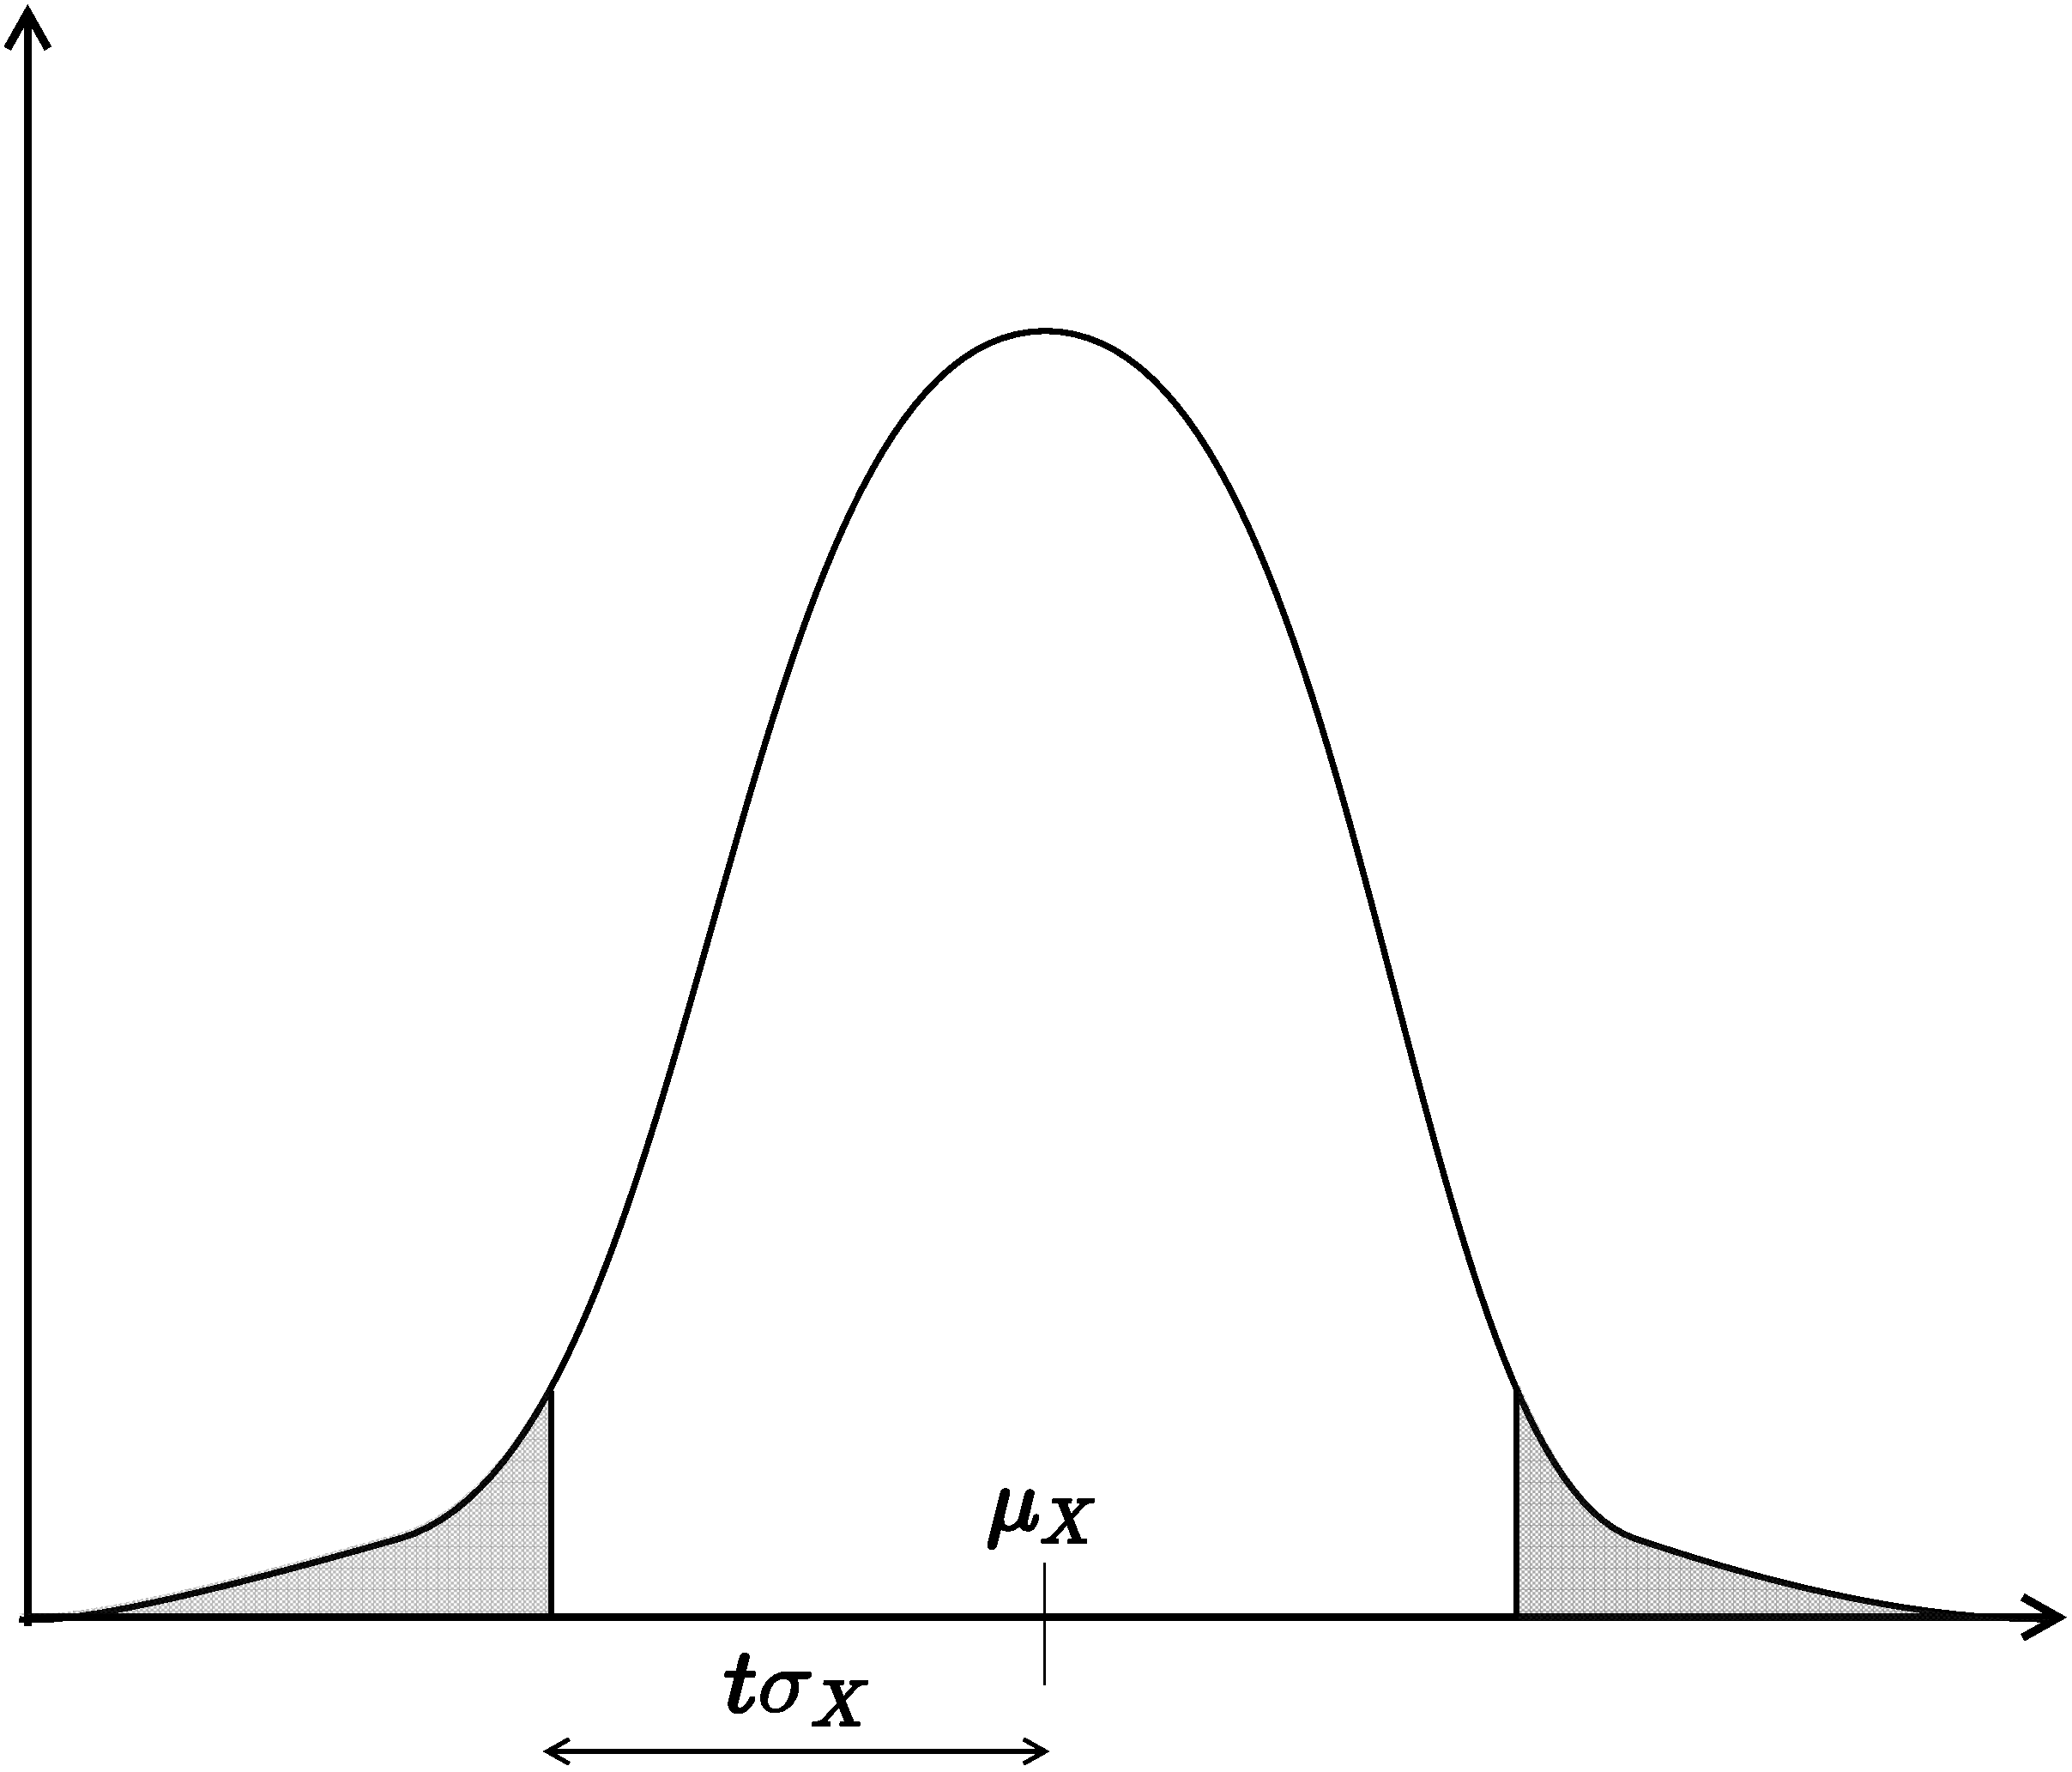
\includegraphics[width=0.4\textwidth]{chebyshev.pdf}
  \end{center}
  \caption{Illustration af Chebyshevs ulighed. Summen af de skraverede områder er $\leq 1/t^2$.}
  \label{fig:chebyshev}
\end{figure}
